\documentclass[11pt,reqno]{amsart}
\usepackage{graphicx}
\usepackage{enumerate}
\usepackage{mathtools}
\usepackage[margin=1in]{geometry}
\usepackage{booktabs}
\usepackage{graphicx}
\usepackage{amsmath}
\usepackage{hyperref}
\usepackage{subcaption} % 导入 subcaption 包以支持子图
\usepackage{float}
\renewcommand{\theequation}{\arabic{enumi}.\arabic{equation}}

\DeclareMathOperator{\im}{im}
\DeclareMathOperator{\rank}{rank}
\DeclareMathOperator{\nullity}{nullity}
\DeclareMathOperator{\tr}{tr}

\newcommand{\tp}{{\scriptscriptstyle\mathsf{T}}}
\usepackage{listings} 
\usepackage{xcolor} 
\lstset{
  language=C++,                 % 设置语言为 C++
  basicstyle=\ttfamily,          % 使用等宽字体
  keywordstyle=\color{blue},     % 关键字高亮为蓝色
  commentstyle=\color{green},    % 注释高亮为绿色
  stringstyle=\color{red},       % 字符串高亮为红色
  numberstyle=\tiny\color{gray}, % 行号高亮为灰色
  numbers=left,                  % 行号显示在左侧
  stepnumber=1,                  % 每行显示行号
  frame=single,                  % 给代码加一个边框
  breaklines=true,               % 自动换行
  backgroundcolor=\color{lightgray!20}, % 设置背景颜色
  captionpos=b,                  % 标题在底部
  showspaces=false,              % 显示空格
  showstringspaces=false,        % 在字符串中显示空格
}
\lstdefinestyle{python}{
    language=Python,
    basicstyle=\ttfamily\small,  % Code font size
    keywordstyle=\bfseries\color{blue},
    commentstyle=\itshape\color{green!50!black},
    stringstyle=\color{orange},
    showstringspaces=false,
    frame=single,                % Adds a border around the code
    numbers=left,                % Line numbers on the left
    numberstyle=\tiny\color{gray},
    breaklines=true,             % Automatic line breaking
    captionpos=b,                % Caption at the bottom
    tabsize=4,                   % Tab size
}
\setlength{\parindent}{0pt}
\begin{document}
\title[]{Project3:Model error correction in ensemble data assimilation\\Chu Zhuyiheng 12455799}
\maketitle


\section{Code framework explanation and result display}

The code \verb|twoccale_ENKF_struct_addNN.py| can draw a picture to compare
the filtering performance of ENKF with and without neural network correction.

\verb|ENKF_class.py| implemented several different ENKFs, and be able to create realistic trajectories and observations using 4th-order Runge–Kutta.

\verb|data_maker.py| is used to produce data by assimilating observations into the single-scale Lorenz96 using an ensemble Kalman filter in order to train the network.

\verb|MLP.py| described the architecture of the network (just an MLP) and can be used to train the network.

\verb|model_80_1500_8.pth| is the best network parameters I trained.

The result is figure~\ref{fig:ENKFs_result}

It can be found that compared with the observed trajectory, ENKF significantly reduces the error, and compared with ENKF, the ENKF using network correction further reduces the error.

\begin{figure}[htbp]
  \centering
      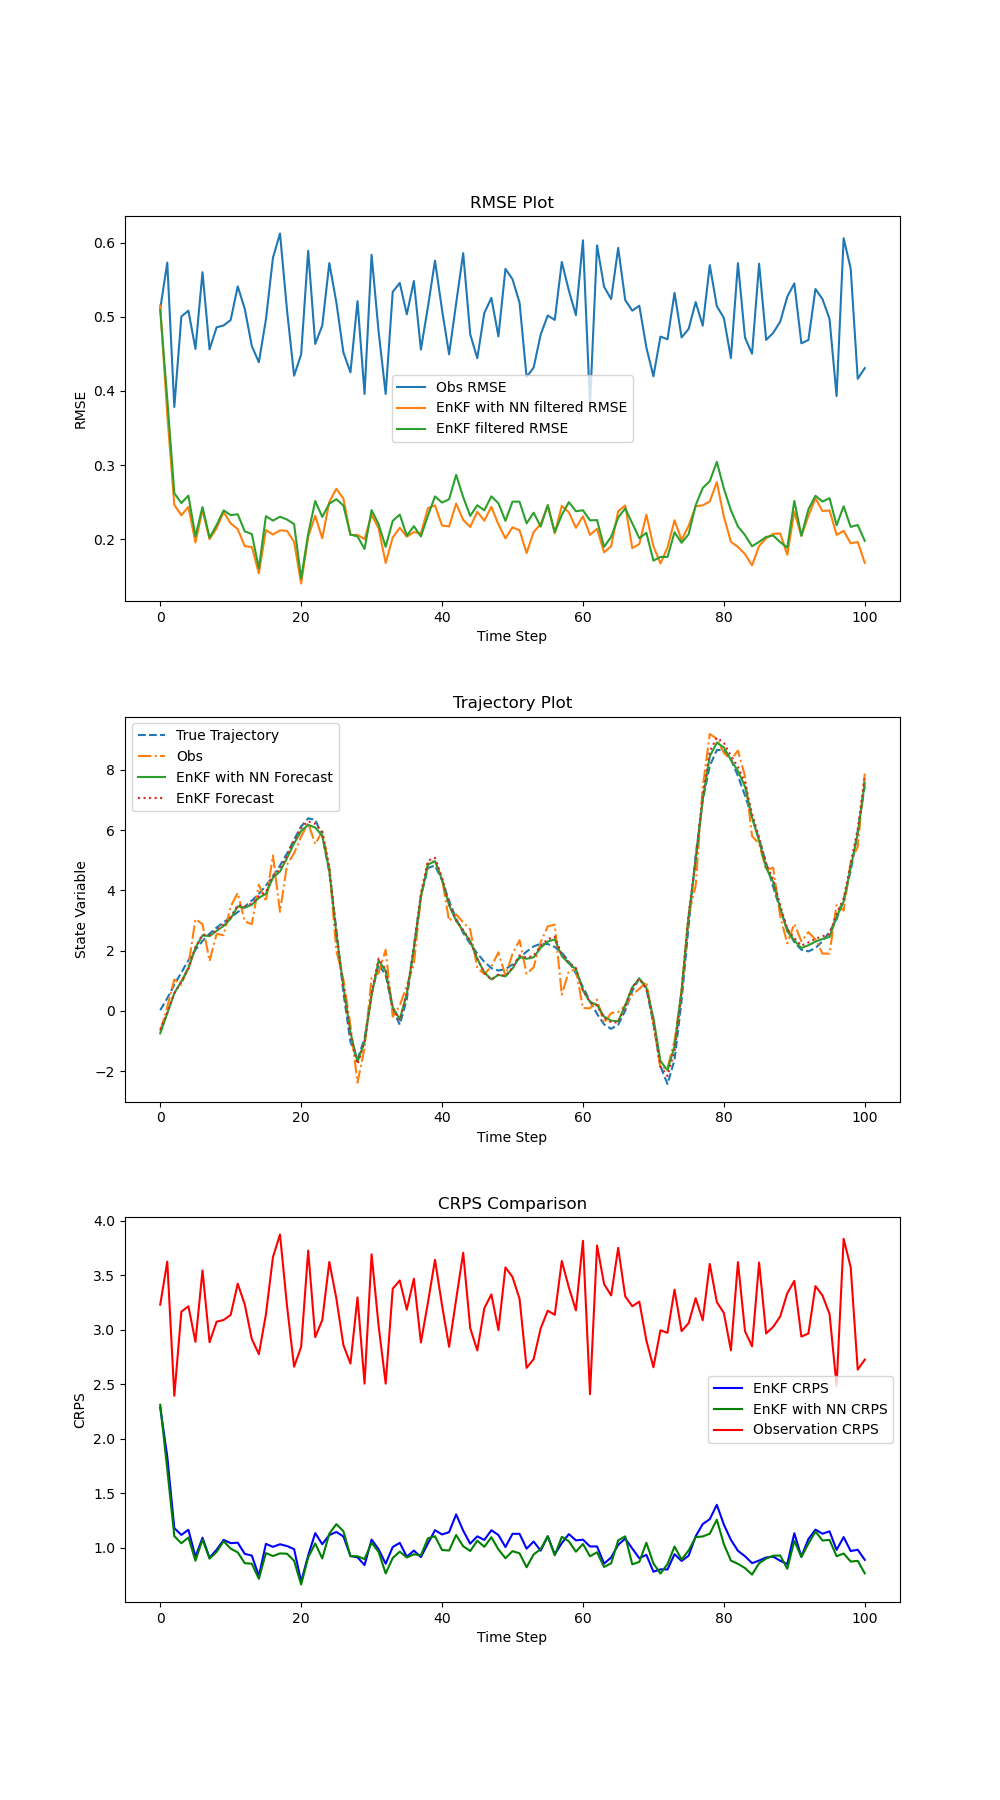
\includegraphics[width=0.8\textwidth]{/mnt/c/workspace/study/Inverse Problem and Data Assimilation/project/Project3/pic/result.png} % Replace with actual image file
      \caption{ENKFs result}
      \label{fig:ENKFs_result}
\end{figure}
\begin{verbatim}
Observation vs True:
RMSE: 0.5322, MAE: 0.4504, Mean CRPS: 3.1714

EnKF Analysis vs True:
RMSE: 0.2072, MAE: 0.1669, Mean CRPS: 1.0355
EnKF with NN Analysis vs True:
RMSE: 0.2032, MAE: 0.1618, Mean CRPS: 0.9819
\end{verbatim}

\section{An attempt at 2 ensembles EnKF}

I found an article~\cite{houtekamer_1998}  mentioned that in order to avoid the rms spread in the ensemble being
 underestimated, two ensembles were used to calculate the covariance matrix and update each other's state, 
 which achieved better results. I tried to use this method instead of the inflation mentioned in the lecture
  notes. Then I got the following results as figure~\ref{fig:2_ensembles_ENKF_result}.

  It can be found that although the effect is not better than ENKF with inflation, it is at least better than the effect without inflation.

  Perhaps when it is not possible to carefully select the inflation parameter, 2 ensembles EnKF would also be a possible option?
  \begin{figure}[htbp]
  \centering
  % Subfigure 1: ML Ensemble Size = 20
  \begin{subfigure}[t]{0.65\textwidth}
      \centering
      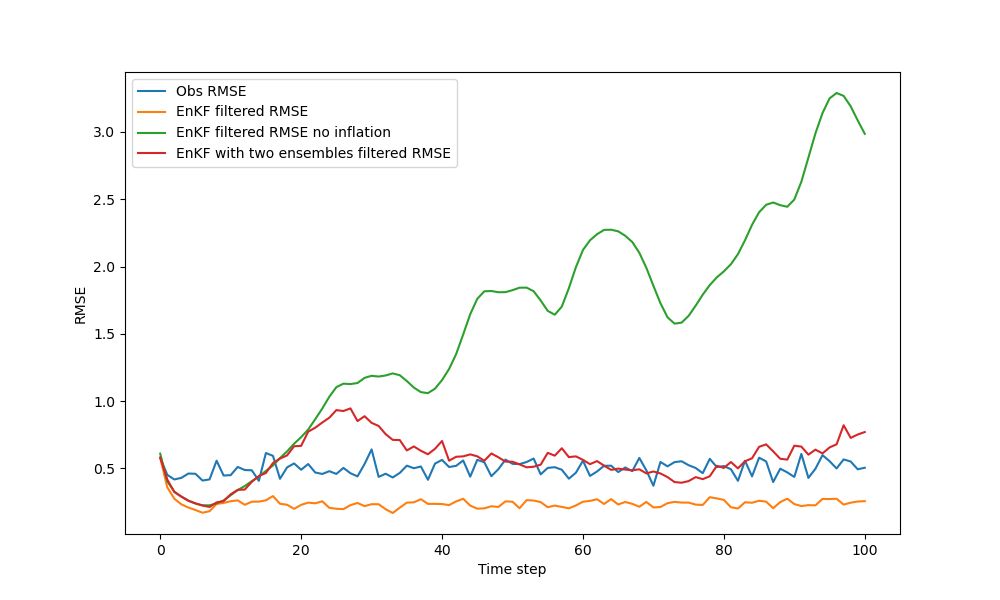
\includegraphics[width=\textwidth]{/mnt/c/workspace/study/Inverse Problem and Data Assimilation/project/Project3/pic/ENKF_inflation.png} % Replace with actual image file
      \caption{RMSE trend}
      \label{fig:ml-ensemble-20}
  \end{subfigure}
  \vspace{0.5cm}
  
  % Subfigure 2: ML Ensemble Size = 50
  \begin{subfigure}[t]{0.65\textwidth}
      \centering
      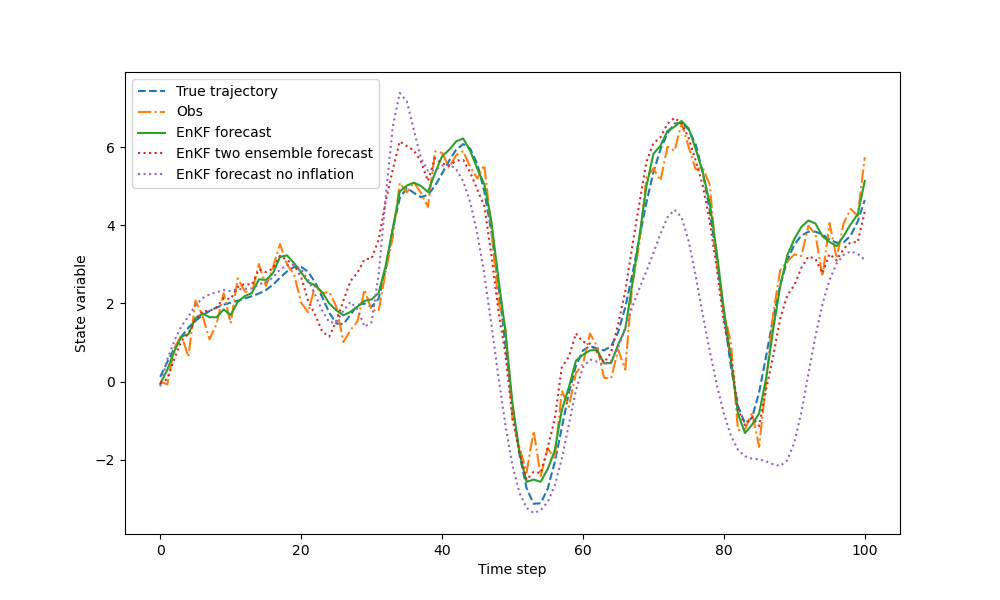
\includegraphics[width=\textwidth]{/mnt/c/workspace/study/Inverse Problem and Data Assimilation/project/Project3/pic/ENKF_inflation_2.png} % Replace with actual image file
      \caption{Dim 0 trend}
      \label{fig:ml-ensemble-50}
  \end{subfigure}
  \vspace{0.5cm}

  \caption{2 ensembles ENKF result}
  \label{fig:2_ensembles_ENKF_result}
\end{figure}

\begin{thebibliography}{9}
  \bibitem{houtekamer_1998}
  Houtekamer, P. L. and Mitchell, H. L. (1998). 
  Data Assimilation Using an Ensemble Kalman Filter Technique. 
  \textit{Monthly Weather Review}, \textit{126}(3), 796--811. 
  \href{https://journals.ametsoc.org/view/journals/mwre/126/3/1520-0493_1998_126_0796_dauaek_2.0.co_2.xml}{link}.
\end{thebibliography}
\end{document}